\chapter{Web Application} \label{Application}

\ifpdf
    \graphicspath{{chapter_7/figures/PNG/}{chapter_7/figures/PDF/}{chapter_7/figures/}}
\else
    \graphicspath{{chapter_7/figures/EPS/}{chapter_7/figures/}}
\fi

\section{Development}

The tool has been developed using flask framework. Flask is a framework of python. With this framework we have used some method of flask like Send, Post, Request and bash scripting. When user submit protein sequence on the input filed flask request helper passes that data to the controller. And using that controller the data is sent to the machine learning algorithm with the help of Post method. After the machine learning processes that data the predicted result is sent to the view/web page with the help of Send method.

\section{User manual}

Visit \url{http://fseacp.pythonanywhere.com} for the home page. After visiting the home page there will be menu buttons for different pages. To detect anticancer peptides go to \url{http://fseacp.pythonanywhere.com/server}. Insert your anticancer peptide sequence you want to predict in the text area as fasta format. After inserting your anticancer peptide sequence you can press clear button to clear out the text area or you can click submit button to check results. After clicking the submit button the input data will be passed to machine learning algorithm using controller and after processing the data then a post method will be sent to the server page with predicted result. If anticancer peptides are detected it send accuracy, "Anti-Cancer Peptide Detected" if not then "No Anticancer Peptides are Detected". If you enter a random string that doesn't match to an anticancer peptide the send response will be "Invalid Sequence". Here we also add some screen-shots. To see the contributors who worked for this tool click on the contributors menu button on the top right corner. To download datasets you can go to \url{http://fseacp.pythonanywhere.com/downloads}. Here we also add read me section \url{http://fseacp.pythonanywhere.com/readme} to make our website more user friendly.
\begin{figure}[H]
\centering
 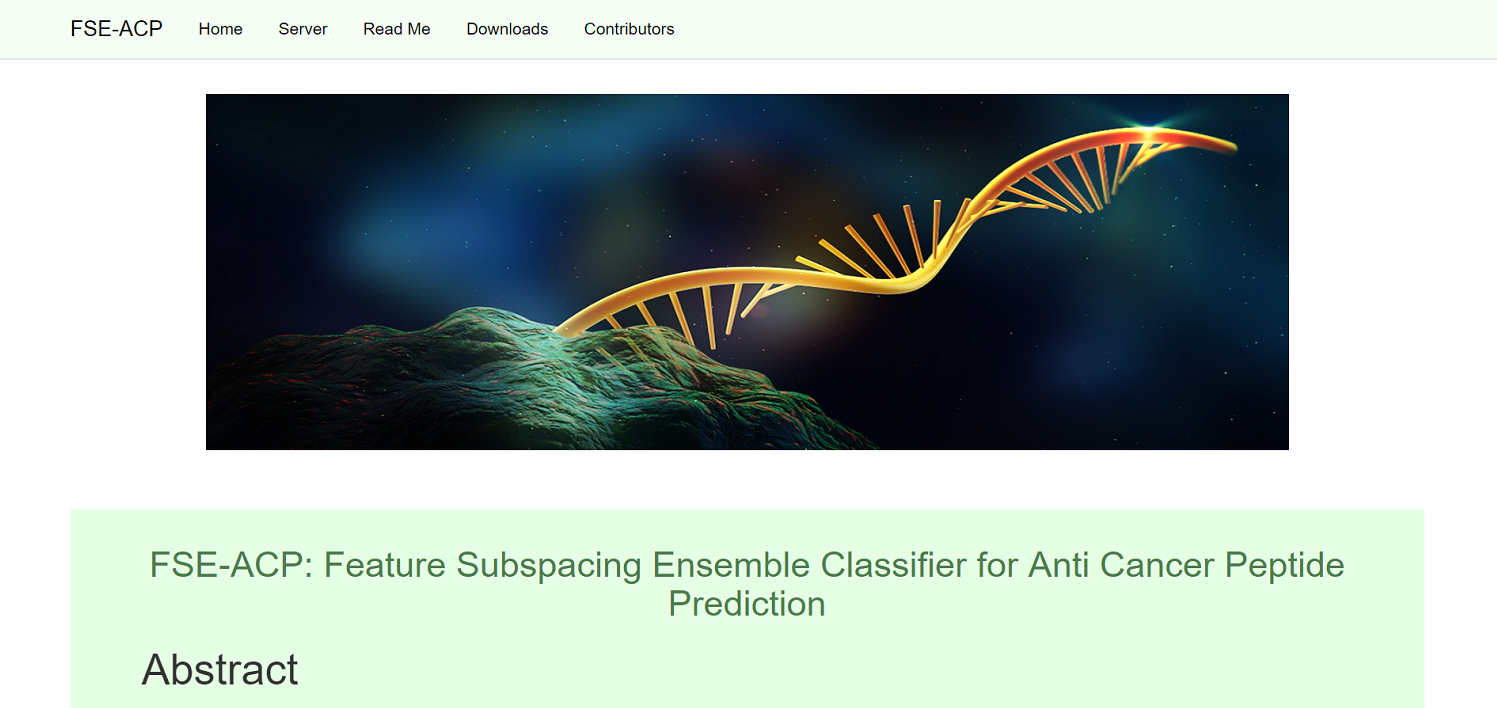
\includegraphics[width=0.8\textwidth]{home.png}
 \caption{Home Page}
\end{figure}
\begin{figure}[H]
\centering
 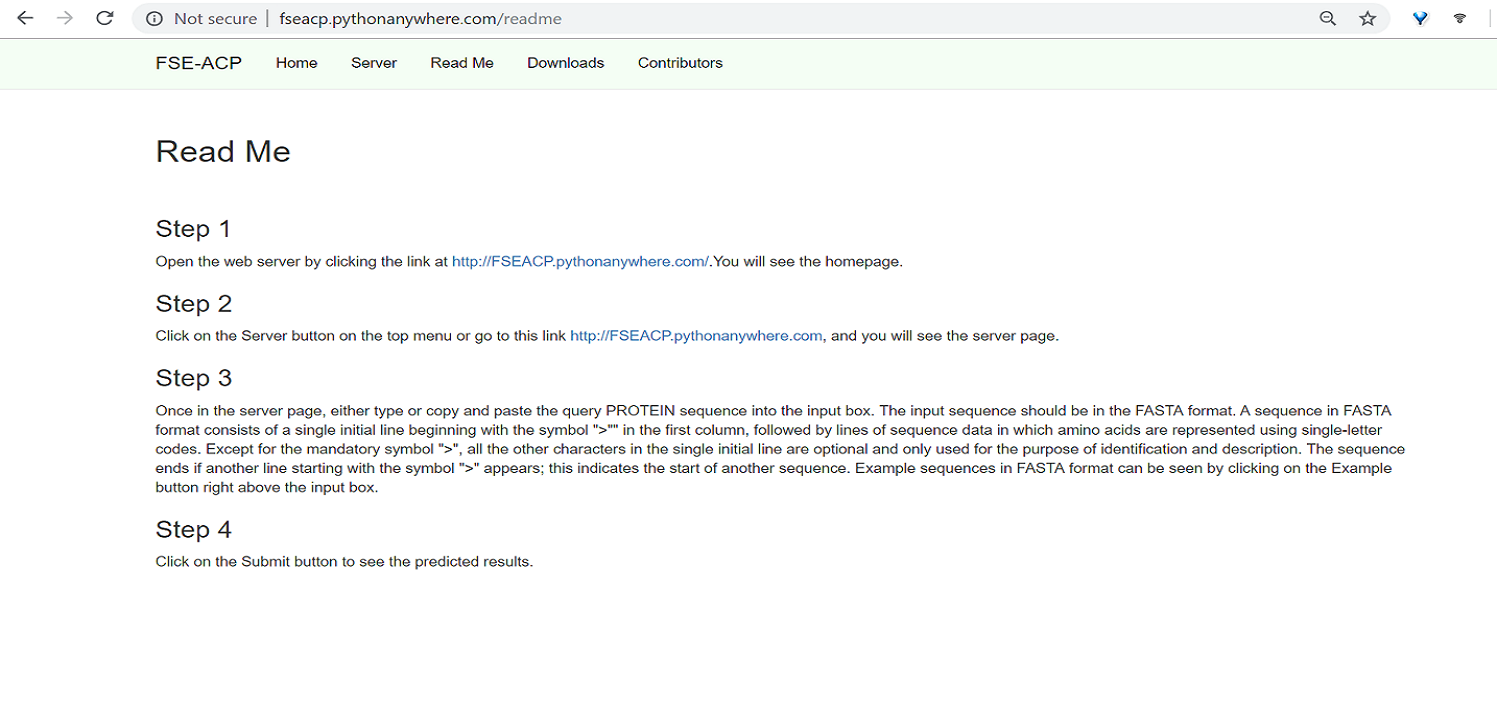
\includegraphics[width=0.8\textwidth]{read.png}
 \caption{Read Me Page}
\end{figure}
\begin{figure}[H]
\centering
 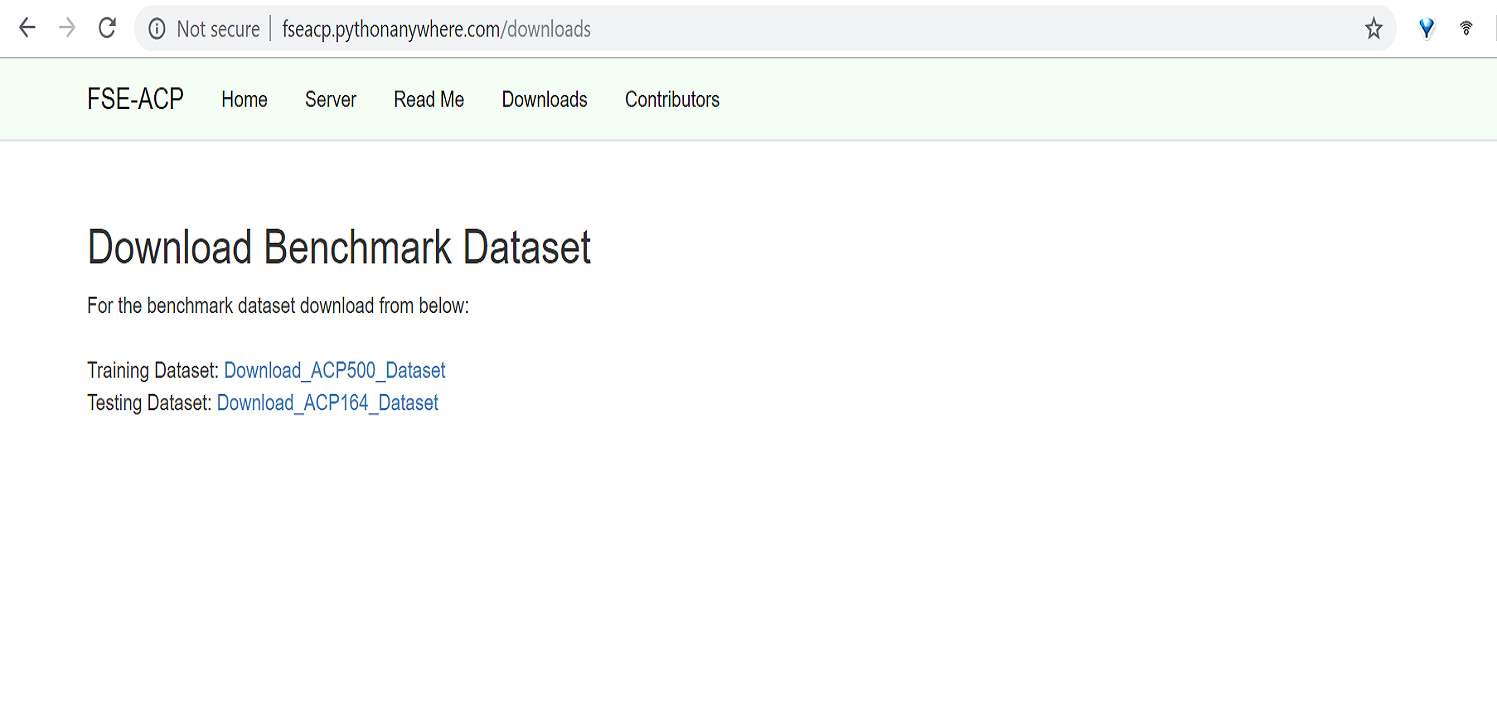
\includegraphics[width=0.8\textwidth]{dataset.png}
 \caption{Downloads Page}
\end{figure}
\begin{figure}[H]
\centering
 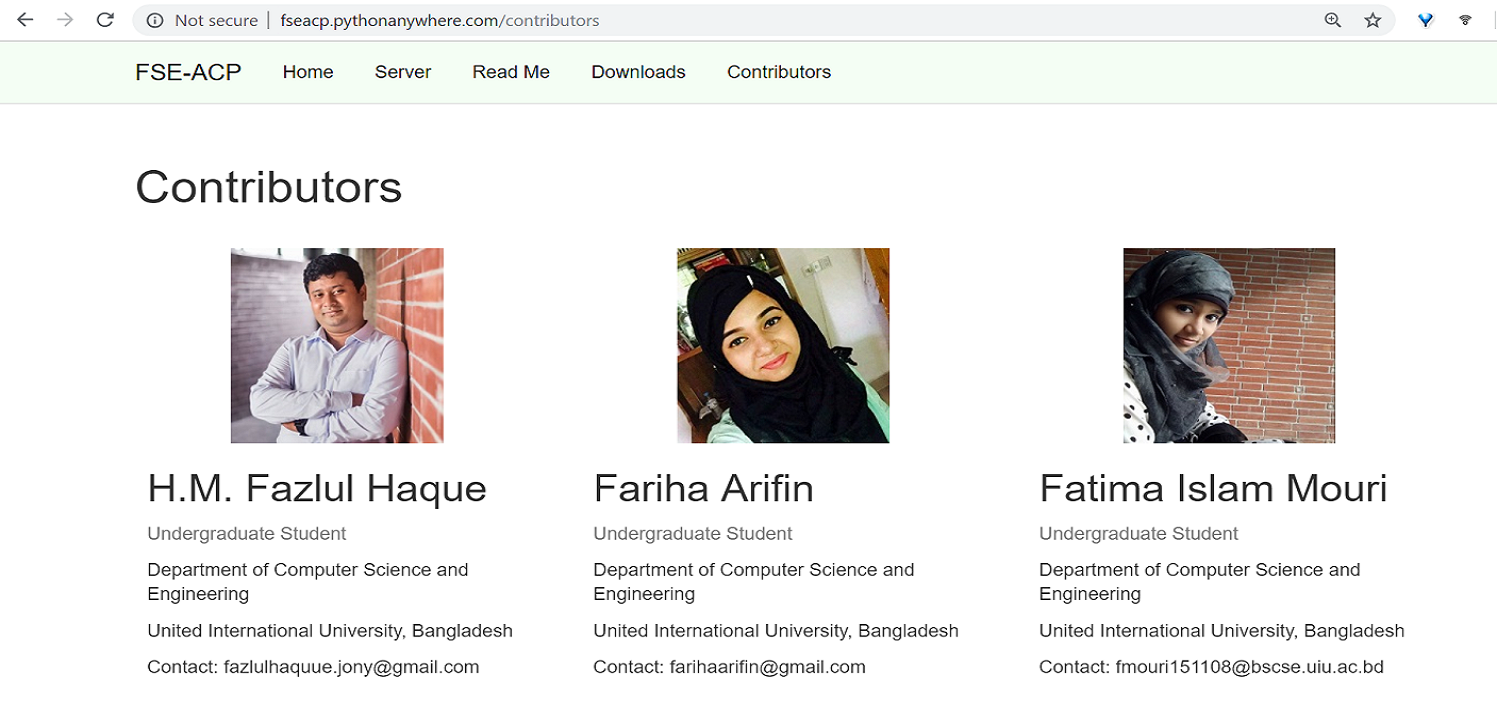
\includegraphics[width=0.8\textwidth]{contri1.png}
 \caption{Contributors Page}
\end{figure}
\begin{figure}[H]
\centering
 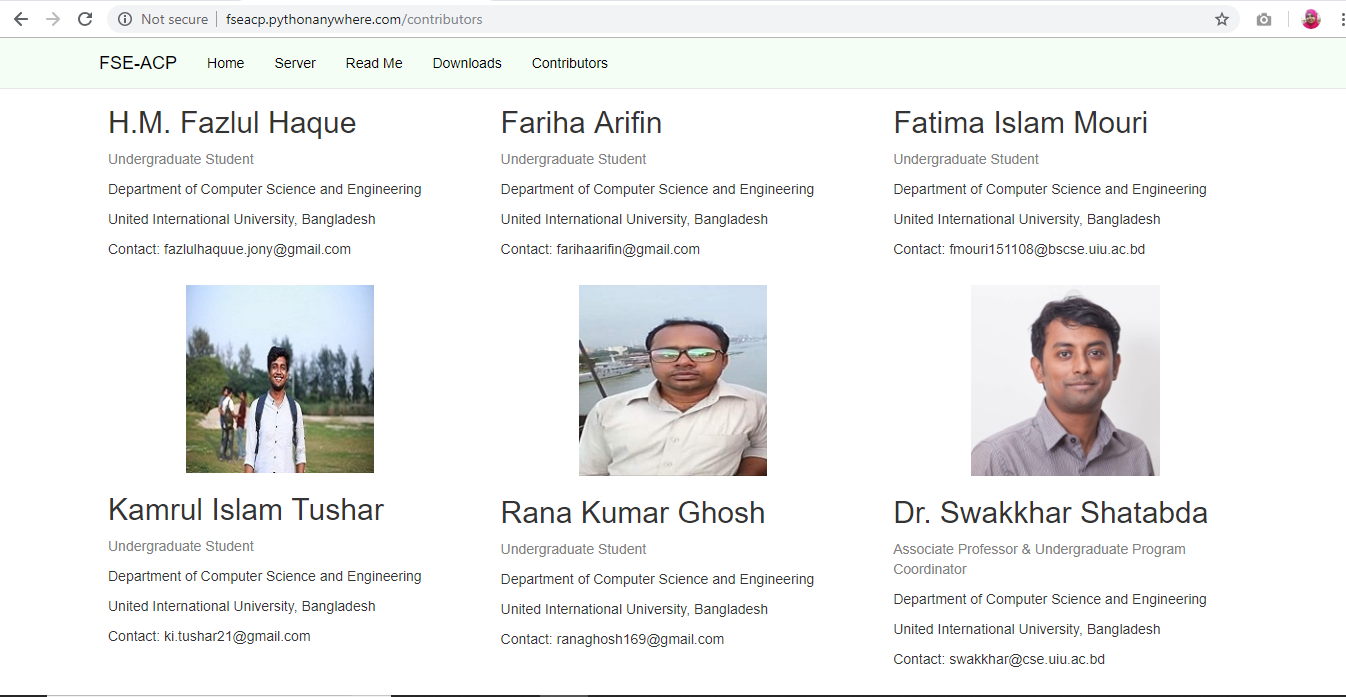
\includegraphics[width=0.8\textwidth]{contri2.png}
 \caption{Contributors Page}
\end{figure}
\begin{figure}[H]
\centering
 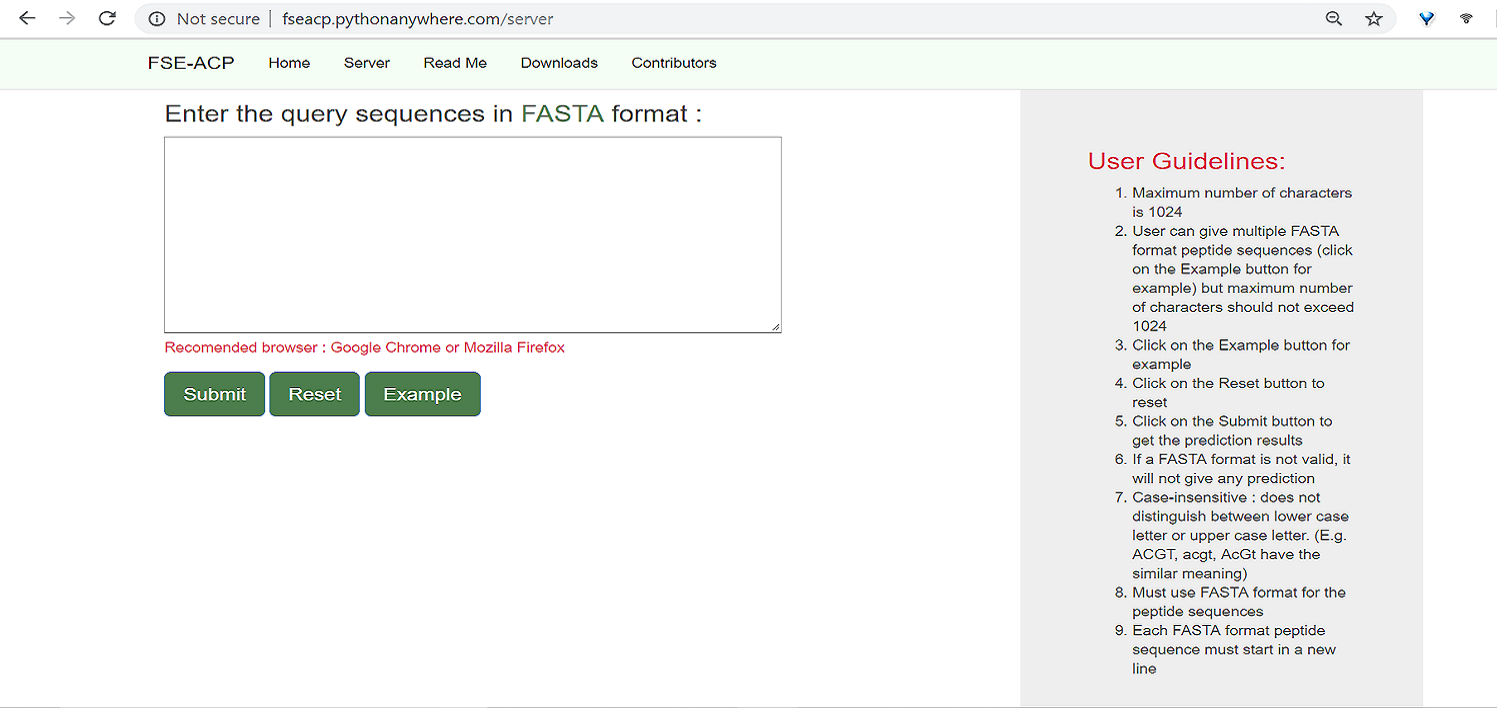
\includegraphics[width=0.8\textwidth]{server1.png}
 \caption{Server main Page}
\end{figure}
\begin{figure}[H]
\centering
 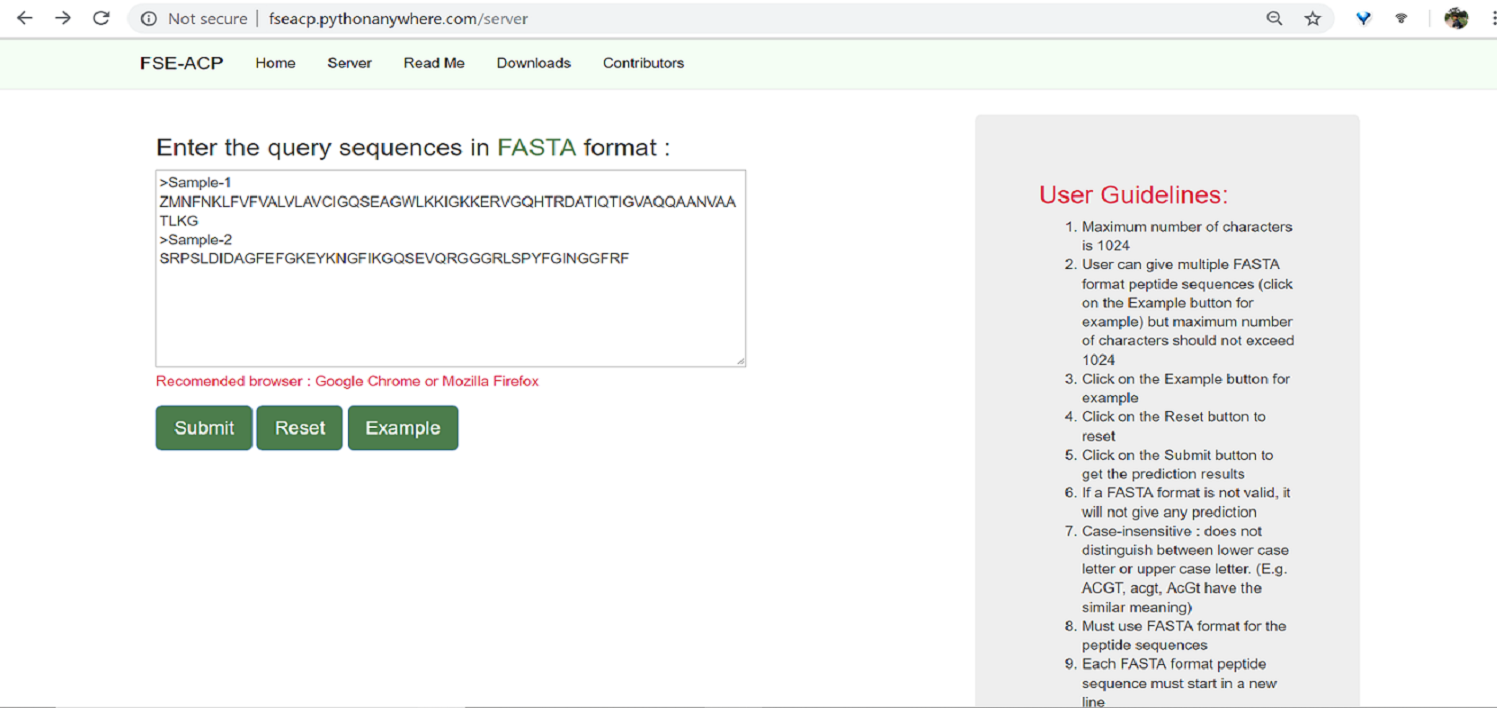
\includegraphics[width=0.8\textwidth]{server2.png}
 \caption{Server Page(with example data)}
\end{figure}
\begin{figure}[H]
\centering
 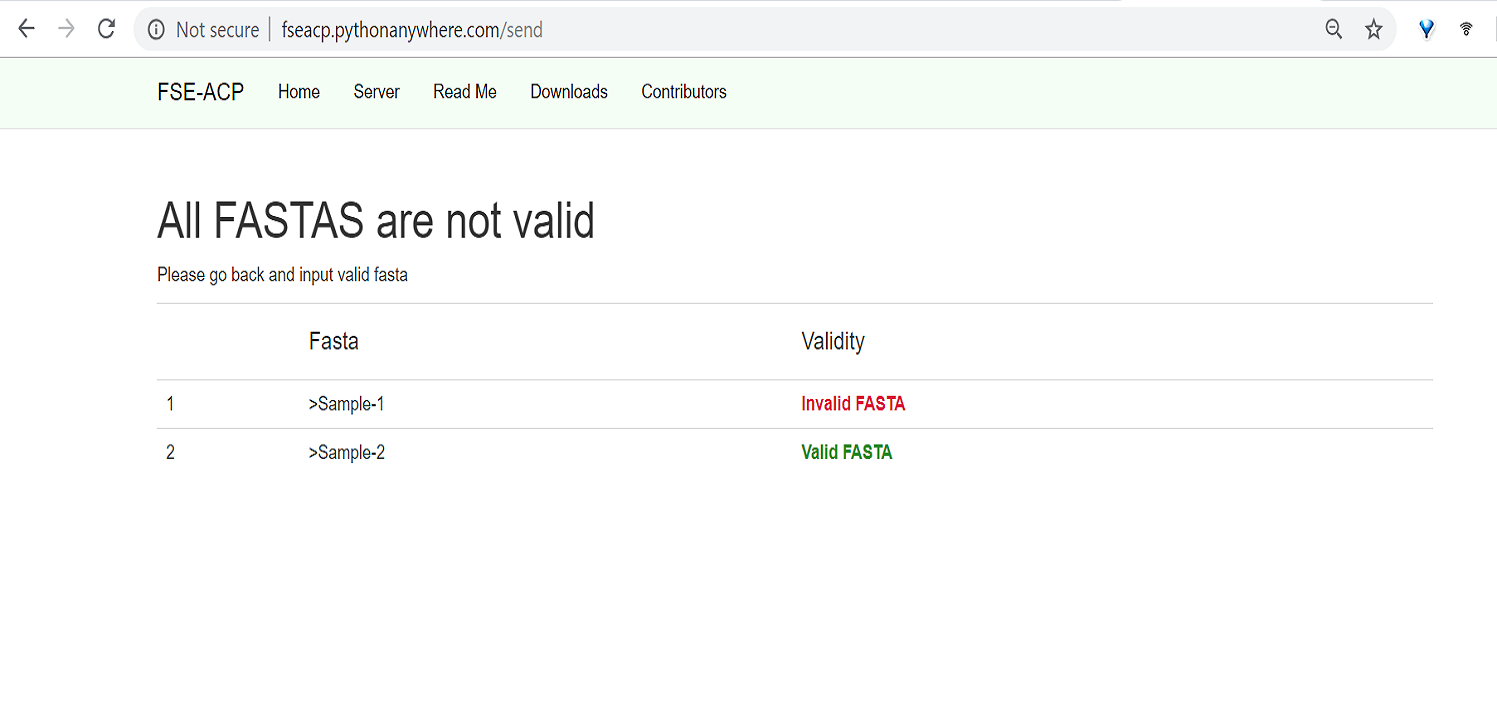
\includegraphics[width=0.8\textwidth]{server3.png}
 \caption{Server Page(result of example data)}
\end{figure}
\begin{figure}[H]
\centering
 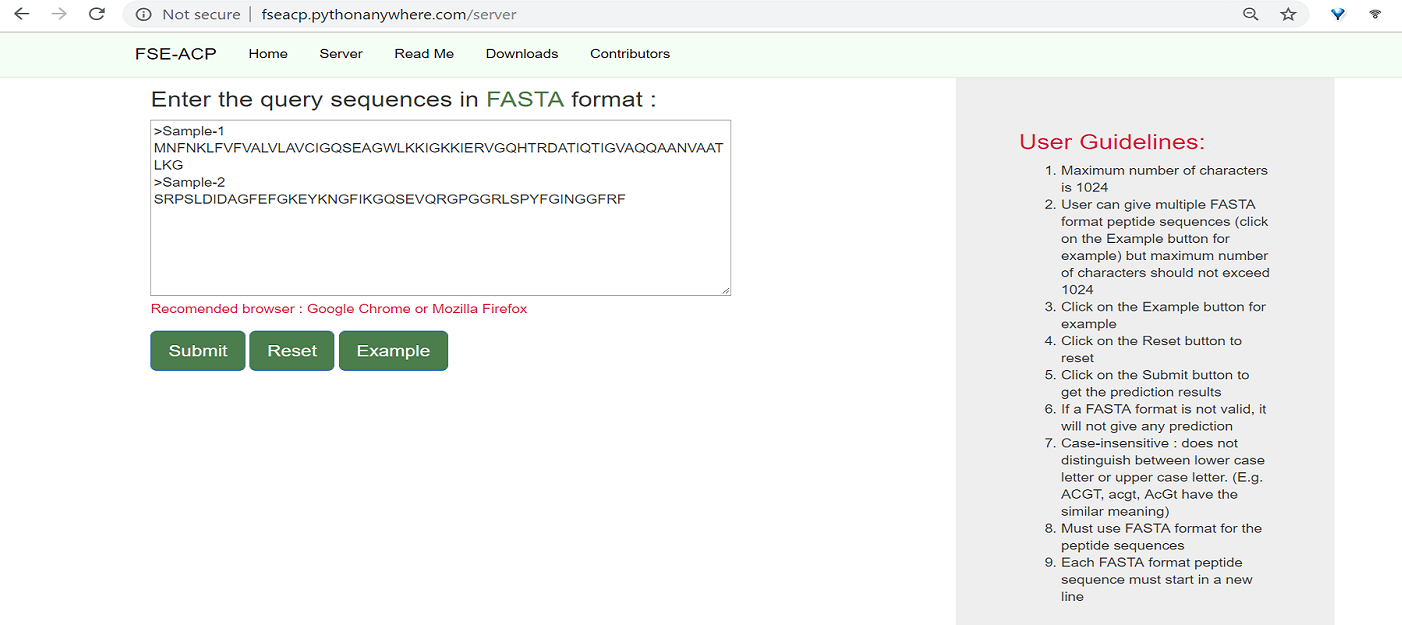
\includegraphics[width=0.8\textwidth]{server4.png}
 \caption{Server Page(with other data)}
\end{figure}
\begin{figure}[H]
\centering
 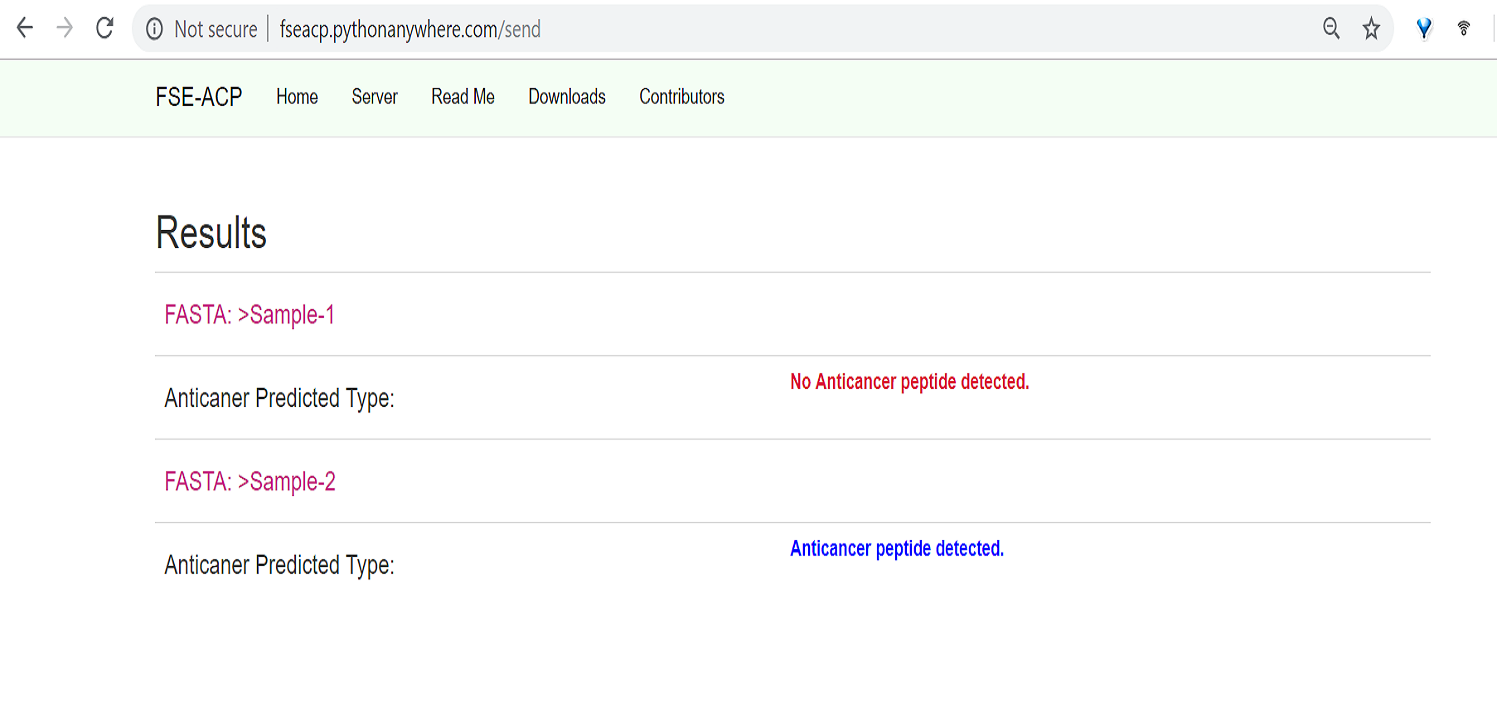
\includegraphics[width=0.8\textwidth]{server5.png}
 \caption{Server Page(result of other data)}
\end{figure}
